
%% bare_conf.tex
%% V1.4b
%% 2015/08/26
%% by Michael Shell
%% See:
%% http://www.michaelshell.org/
%% for current contact information.
%%
%% This is a skeleton file demonstrating the use of IEEEtran.cls
%% (requires IEEEtran.cls version 1.8b or later) with an IEEE
%% conference paper.
%%
%% Support sites:
%% http://www.michaelshell.org/tex/ieeetran/
%% http://www.ctan.org/pkg/ieeetran
%% and
%% http://www.ieee.org/

%%*************************************************************************
%% Legal Notice:
%% This code is offered as-is without any warranty either expressed or
%% implied; without even the implied warranty of MERCHANTABILITY or
%% FITNESS FOR A PARTICULAR PURPOSE! 
%% User assumes all risk.
%% In no event shall the IEEE or any contributor to this code be liable for
%% any damages or losses, including, but not limited to, incidental,
%% consequential, or any other damages, resulting from the use or misuse
%% of any information contained here.
%%
%% All comments are the opinions of their respective authors and are not
%% necessarily endorsed by the IEEE.
%%
%% This work is distributed under the LaTeX Project Public License (LPPL)
%% ( http://www.latex-project.org/ ) version 1.3, and may be freely used,
%% distributed and modified. A copy of the LPPL, version 1.3, is included
%% in the base LaTeX documentation of all distributions of LaTeX released
%% 2003/12/01 or later.
%% Retain all contribution notices and credits.
%% ** Modified files should be clearly indicated as such, including  **
%% ** renaming them and changing author support contact information. **
%%*************************************************************************

% *** Authors should verify (and, if needed, correct) their LaTeX system  ***
% *** with the testflow diagnostic prior to trusting their LaTeX platform ***
% *** with production work. The IEEE's font choices and paper sizes can   ***
% *** trigger bugs that do not appear when using other class files.       ***                          ***
% The testflow support page is at:
% http://www.michaelshell.org/tex/testflow/

\documentclass[conference]{IEEEtran}
% Some Computer Society conferences also require the compsoc mode option,
% but others use the standard conference format.
%
% If IEEEtran.cls has not been installed into the LaTeX system files,
% manually specify the path to it like:
% \documentclass[conference]{../sty/IEEEtran}

% Some very useful LaTeX packages include:
% (uncomment the ones you want to load)

% *** MISC UTILITY PACKAGES ***
%
%\usepackage{ifpdf}
% Heiko Oberdiek's ifpdf.sty is very useful if you need conditional
% compilation based on whether the output is pdf or dvi.
% usage:
% \ifpdf
%   % pdf code
% \else
%   % dvi code
% \fi
% The latest version of ifpdf.sty can be obtained from:
% http://www.ctan.org/pkg/ifpdf
% Also, note that IEEEtran.cls V1.7 and later provides a builtin
% \ifCLASSINFOpdf conditional that works the same way.
% When switching from latex to pdflatex and vice-versa, the compiler may
% have to be run twice to clear warning/error messages.

% *** CITATION PACKAGES ***
%
\usepackage{cite}

% *** GRAPHICS RELATED PACKAGES ***
%
\ifCLASSINFOpdf
 \usepackage[pdftex]{graphicx}
  % declare the path(s) where your graphic files are
  % \graphicspath{{../pdf/}{../jpeg/}}
  % and their extensions so you won't have to specify these with
  % every instance of \includegraphics
  % \DeclareGraphicsExtensions{.pdf,.jpeg,.png}
\else
  % or other class option (dvipsone, dvipdf, if not using dvips). graphicx
  % will default to the driver specified in the system graphics.cfg if no
  % driver is specified.
  % \usepackage[dvips]{graphicx}
  % declare the path(s) where your graphic files are
  % \graphicspath{{../eps/}}
  % and their extensions so you won't have to specify these with
  % every instance of \includegraphics
  % \DeclareGraphicsExtensions{.eps}
\fi
% graphicx was written by David Carlisle and Sebastian Rahtz. It is
% required if you want graphics, photos, etc. graphicx.sty is already
% installed on most LaTeX systems. The latest version and documentation
% can be obtained at: 
% http://www.ctan.org/pkg/graphicx
% Another good source of documentation is "Using Imported Graphics in
% LaTeX2e" by Keith Reckdahl which can be found at:
% http://www.ctan.org/pkg/epslatex
%
% latex, and pdflatex in dvi mode, support graphics in encapsulated
% postscript (.eps) format. pdflatex in pdf mode supports graphics
% in .pdf, .jpeg, .png and .mps (metapost) formats. Users should ensure
% that all non-photo figures use a vector format (.eps, .pdf, .mps) and
% not a bitmapped formats (.jpeg, .png). The IEEE frowns on bitmapped formats
% which can result in "jaggedy"/blurry rendering of lines and letters as
% well as large increases in file sizes.
%
% You can find documentation about the pdfTeX application at:
% http://www.tug.org/applications/pdftex

% *** MATH PACKAGES ***
%
\usepackage{amsmath}

% *** SPECIALIZED LIST PACKAGES ***
%
%\usepackage{algorithmic}

% *** ALIGNMENT PACKAGES ***
%
%\usepackage{array}


% IEEEtran contains the IEEEeqnarray family of commands that can be used to
% generate multiline equations as well as matrices, tables, etc., of high
% quality.

% *** SUBFIGURE PACKAGES ***
\ifCLASSOPTIONcompsoc
  \usepackage[caption=false,font=normalsize,labelfont=sf,textfont=sf]{subfig}
\else
  \usepackage[caption=false,font=footnotesize]{subfig}
\fi
% subfig.sty, written by Steven Douglas Cochran, is the modern replacement
% for subfigure.sty, the latter of which is no longer maintained and is
% incompatible with some LaTeX packages including fixltx2e. However,
% subfig.sty requires and automatically loads Axel Sommerfeldt's caption.sty
% which will override IEEEtran.cls' handling of captions and this will result
% in non-IEEE style figure/table captions. To prevent this problem, be sure
% and invoke subfig.sty's "caption=false" package option (available since
% subfig.sty version 1.3, 2005/06/28) as this is will preserve IEEEtran.cls
% handling of captions.
% Note that the Computer Society format requires a larger sans serif font
% than the serif footnote size font used in traditional IEEE formatting
% and thus the need to invoke different subfig.sty package options depending
% on whether compsoc mode has been enabled.
%
% The latest version and documentation of subfig.sty can be obtained at:
% http://www.ctan.org/pkg/subfig




% *** FLOAT PACKAGES ***
%
%\usepackage{fixltx2e}
% fixltx2e, the successor to the earlier fix2col.sty, was written by
% Frank Mittelbach and David Carlisle. This package corrects a few problems
% in the LaTeX2e kernel, the most notable of which is that in current
% LaTeX2e releases, the ordering of single and double column floats is not
% guaranteed to be preserved. Thus, an unpatched LaTeX2e can allow a
% single column figure to be placed prior to an earlier double column
% figure.
% Be aware that LaTeX2e kernels dated 2015 and later have fixltx2e.sty's
% corrections already built into the system in which case a warning will
% be issued if an attempt is made to load fixltx2e.sty as it is no longer
% needed.
% The latest version and documentation can be found at:
% http://www.ctan.org/pkg/fixltx2e


%\usepackage{stfloats}
% stfloats.sty was written by Sigitas Tolusis. This package gives LaTeX2e
% the ability to do double column floats at the bottom of the page as well
% as the top. (e.g., "\begin{figure*}[!b]" is not normally possible in
% LaTeX2e). It also provides a command:
%\fnbelowfloat
% to enable the placement of footnotes below bottom floats (the standard
% LaTeX2e kernel puts them above bottom floats). This is an invasive package
% which rewrites many portions of the LaTeX2e float routines. It may not work
% with other packages that modify the LaTeX2e float routines. The latest
% version and documentation can be obtained at:
% http://www.ctan.org/pkg/stfloats
% Do not use the stfloats baselinefloat ability as the IEEE does not allow
% \baselineskip to stretch. Authors submitting work to the IEEE should note
% that the IEEE rarely uses double column equations and that authors should try
% to avoid such use. Do not be tempted to use the cuted.sty or midfloat.sty
% packages (also by Sigitas Tolusis) as the IEEE does not format its papers in
% such ways.
% Do not attempt to use stfloats with fixltx2e as they are incompatible.
% Instead, use Morten Hogholm'a dblfloatfix which combines the features
% of both fixltx2e and stfloats:
%
% \usepackage{dblfloatfix}
% The latest version can be found at:
% http://www.ctan.org/pkg/dblfloatfix




% *** PDF, URL AND HYPERLINK PACKAGES ***
%
%\usepackage{url}
% url.sty was written by Donald Arseneau. It provides better support for
% handling and breaking URLs. url.sty is already installed on most LaTeX
% systems. The latest version and documentation can be obtained at:
% http://www.ctan.org/pkg/url
% Basically, \url{my_url_here}.




% *** Do not adjust lengths that control margins, column widths, etc. ***
% *** Do not use packages that alter fonts (such as pslatex).         ***
% There should be no need to do such things with IEEEtran.cls V1.6 and later.
% (Unless specifically asked to do so by the journal or conference you plan
% to submit to, of course. )


% correct bad hyphenation here
\hyphenation{op-tical net-works semi-conduc-tor}


\begin{document}
%
% paper title
% Titles are generally capitalized except for words such as a, an, and, as,
% at, but, by, for, in, nor, of, on, or, the, to and up, which are usually
% not capitalized unless they are the first or last word of the title.
% Linebreaks \\ can be used within to get better formatting as desired.
% Do not put math or special symbols in the title.
\title{Deep Reinforcement Learning for Browser Tasks}


% author names and affiliations
% use a multiple column layout for up to three different
% affiliations
\author{\IEEEauthorblockN{Minttu Alakuijala\IEEEauthorrefmark{1}}
\IEEEauthorblockA{minttu.alakuijala.14@ucl.ac.uk}\\
\IEEEauthorblockN{Jamie Law\IEEEauthorrefmark{1}}
\IEEEauthorblockA{jamie.law.14@ucl.ac.uk}
\and
\IEEEauthorblockN{Vika Christy\IEEEauthorrefmark{1}}
\IEEEauthorblockA{anastasia.christy.14@ucl.ac.uk}\\
\IEEEauthorblockN{Yuhang Xu\IEEEauthorrefmark{1}}
\IEEEauthorblockA{yuhang.xu.14@ucl.ac.uk}\\
\IEEEauthorblockA{\IEEEauthorrefmark{1}University College London, Computer Science}
\and
\IEEEauthorblockN{Rajind Karunaratne\IEEEauthorrefmark{1}}
\IEEEauthorblockA{rajind.karunaratne.14@ucl.ac.uk}\\
\IEEEauthorblockN{Jun Wang\IEEEauthorrefmark{1}}
\IEEEauthorblockA{j.wang@cs.ucl.ac.uk}
}




% use for special paper notices
%\IEEEspecialpapernotice{(Invited Paper)}




% make the title area
\maketitle

% As a general rule, do not put math, special symbols or citations
% in the abstract
\begin{abstract}
Deep learning is an emerging field that has shown many breakthroughs recently due to the technology available. Within reinforcement learning, deep learning has shown to be effective in game-like environments. The purpose of this study is to investigate the effectiveness of using deep reinforcement learning to train agents on a novel benchmark, Mini World of Bits (developed by OpenAI). This benchmark can be seen as an initial foundation for website interaction which, if mastered, would strongly infer development towards performing automation on tasks in real-world websites and furthering progress towards AI general intelligence. We look at adapting and evaluating deep Q-networks and policy gradient algorithms for this benchmark and then determining each model's success based off an average of the reward function from the environments, ideally looking towards a positive trend through the training process. [potential conclusion based on results]
\end{abstract}

% no keywords
% For peer review papers, you can put extra information on the cover
% page as needed:
% \ifCLASSOPTIONpeerreview
% \begin{center} \bfseries EDICS Category: 3-BBND \end{center}
% \fi
%
% For peerreview papers, this IEEEtran command inserts a page break and
% creates the second title. It will be ignored for other modes.
\IEEEpeerreviewmaketitle

\section{Introduction}
Over the past few years, there has been a monumental shift in technology and how it's being applied to everyday life, of which deep reinforcement learning is a field which has recently shown potential due to the technology available. With typical algorithms, computers are told how to deal with problems, but with deep learning computers are told to teach themselves to deal with these problems. Significant progress has already been demonstrated in experiments on the Universe platform, where agents have been trained via deep reinforcement learning to successfully play Atari games \cite{mnih2013playing}. We have looked to extend the implementation of deep reinforcement learning methods onto browser-based tasks. This introduction will give the reader an insight into the concerned technologies as well as deriving a justified hypothesis. 

\subsection{OpenAI Universe}
Universe is a software platform developed by OpenAI built for training and measuring AI across a wide range of games, websites and other environments. Any program can be turned into a Gym (a toolkit for developing and comparing reinforcement learning algorithms) environment via this platform. It provides the agent's access to programs via a VNC client on a remote desktop (inside a Docker container), allowing the agent to perceive and act on the program the same way a human does by interpreting the pixel values of a screen and producing a combination of keyboard and/or mouse actions. 

The ultimate goal of Universe is to develop a single agent that can apply all of its previous experiences to quickly adapt and master to other unfamiliar environments, which would demonstrate monumental progress towards general intelligence. This differs to other systems which typically fall into the category of "Narrow AI", which are systems that perform well in a specific domain but struggle to adapt to other environments. 

A large number of environments have already been integrated into Universe, such as Atari games, Flash games and Browser based tasks, of which a prominent benchmark is Mini World of Bits.

\subsection{Mini World of Bits}

\begin{figure*}[t]
	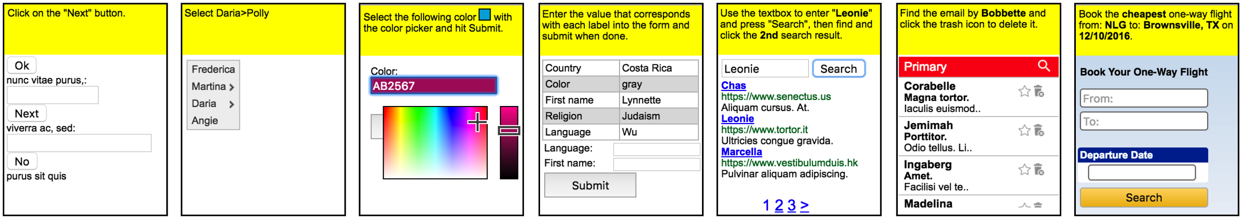
\includegraphics[width=\textwidth, height=\textheight, keepaspectratio]{mwob.png}
	\caption{Example environments from the Mini World of Bits benchmark \cite{mwob}, task prompts are indicated in the yellow section while the white section is the canvas area}
	\label{fig:mwob}
\end{figure*}

Mini World of Bits (MWoB) \cite{mwob} is a new benchmark which consists of a wide range of browser-based tasks, such as clicking a button, entering text, all the way up to more complex tasks such as searching for a flight between dates. It can be seen as an initial foundation that encapsulates the core functionalities of website interactions which, if mastered, would provide strong inference of development towards performing well on real-world websites. The benchmark can be seen as an equivalence to the MNIST dataset \cite{lecun1998gradient} in terms of visual recognition, where the ultimate goal for the agents is to be able to perceive and interpret the provided data in a small, self-contained area to complete the task.

The benchmark consists of 80 environments, which are written in a combination of HTML, JavaScript and CSS, although the agents can not perceive this information via Universe. Each environment is a 210px by 160px webpage, where the yellow section indicates the task prompt and the white section is the canvas area for performing the task (examples of environments can be seen in figure \ref{fig:mwob}). The agents receive visual information which are the raw pixel values of the webpage and then attempt to produce a combination of keyboard or mouse actions to attempt to complete the task. They also receive a reward value based on the task progress, ranging 0 to 1 if the task is completed (dependent on the time taken for completion) and -1 if the task is failed or time has run out.

We have looked into the MWoB benchmark due to its novelty; no results have been published yet for this, in contrast to other Universe environments such as Atari games or Flash games where significant progress has already been demonstrated using deep reinforcement learning \cite{mnih2013playing}.

\subsection{Hypothesis}
Due to the success of deep reinforcement learning in other experiments, we are looking to investigate the effectiveness of using the respective algorithms on the Mini World of Bits benchmark:
\begin{center}
\textit{"Deep Reinforcement Learning would be effective in the Mini World of Bits benchmark"}
\end{center}

\section{Related work}
Subsection text here.

\section{Methodology}

\subsection{Environments}
Due to time restriction, we had to be selective on choosing some of the MWoB environments that we were going to be experimented with. There exist four types of environment such as click tasks, drag tasks, mouse tasks and other tasks. In this research, the main goal is to tackle the click tasks problems. Within the click tasks problem, we eliminated some of the environments that require Natural Language Processing such as \textit{"word-matching"} or \textit{"colour-matching"} as it would be more difficult to develop. At the end, three environments were chosen; click the button, focus into the textbox, and close the dialog box.
\begin{figure}
	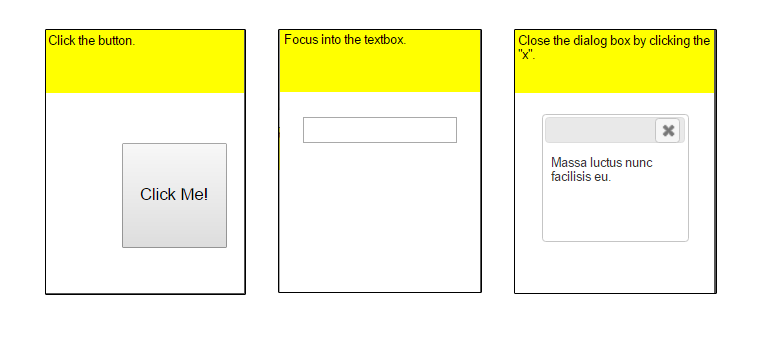
\includegraphics[width=\linewidth]{chosen-envi.png}
	\caption{Environment of: 1. Click The Button, 2. Focus Into The Textbox, 3. Close The Dialog Box}
	\label{fig:chosen-envi}
\end{figure}
\subsection{Action spaces}
An agent performs a series of actions to interact with the environment in hopes of obtaining a reward signal, with the primary objective of maximizing the cumulative reward based on the current state of the environment. When we consider the set of actions an agent is allowed to perform, this set can either be \textbf{discrete} or \textbf{continuous}. A discrete action space is simply a fixed set of actions that an agent is can perform. Continuous action spaces are more complex, often involving function approximations to determine an approximation of the optimal action for a given state. \linebreak

A feature of the Universe platform allows agents to utilize a full set of keyboard presses and mouse controls as part of their action space. When we consider the dynamic nature of the environments, this presents a continuous set of state spaces over time. However regardless of what the task an agent is set out to do, we can determine a generalization to the standard actions an agent would likely perform within the scope of browser-based tasks. When we consider conventional human behavior, controlling \textit{mouse-based} applications often involve the use of moving the cursor in a sequence of directions and clicking upon their target of interest. If we were to discretize this representation for a set of actions at any given frame in time, the cursor can either move in four basic directions (up, down, left, right), click on the spot, or do nothing at all. This interpretation of a discrete action space was our initial starting point for the agent. As this involves sole emphasis on mouse-based tasks, we omit the use of keyboard presses completely, and scale down the testing grounds of our agents to environments that require completion of tasks using mouse-controls only. \linebreak

Of course, the above interpretation completely omits many other factors that build upon the reality of controlling browser-based applications. For example, we do not consider angular directions, dragging actions, or scroll actions to navigate through pages to find elements of interest. Also, discretization of action spaces are poor solutions when it comes to scalability. For example, it?s easy to determine a more efficient solution for a cursor to simple ?warp? to a point in the canvas (similar to an individual clicking a point within a touchscreen). However when we consider the scale of the canvas having dimensions of 160x160 pixels (25,600 possible cursor positions), to discretize this space of pixels can be inefficient and computationally expensive, and thus approximating this space using continuous action spaces is a more efficient solution if we were to consider this approach. However realistically, a majority of conventional browser tasks often require contextual awareness of the tasks to be performed rather than the actions themselves, where our approach first determines the basic foundations of movement and control where such complexities can later be built upon.

\subsection{Input processing}
Generated states of any environment within Universe are represented as raw pixel data, which serve as the primary source of visual context for any agent. As this would be the sole means of supervision used for the training process of the agent itself, we sought to investigate additional techniques to manipulate this data that could help provide an increase in efficiency during training. Some general methods, such as converting images to from RGB to grayscale for environments that did not require color co-ordination and downsampling images to half its size decreased the amount of computation required for an agent to interpret the pixels. However, more complex additions were added to the pixel data with the aim of providing increased contextual awareness for the agent to learn from. \linebreak
\begin{figure}[h!]
\centering
	\subfloat{%
	\begin{minipage}[b][8cm][t]{.2\textwidth}
	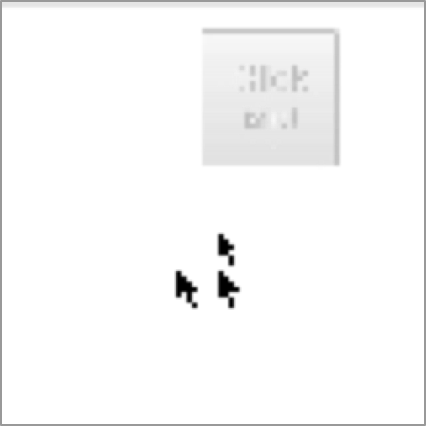
\includegraphics[width=0.9\columnwidth]{downsample.png}
	\vfill
	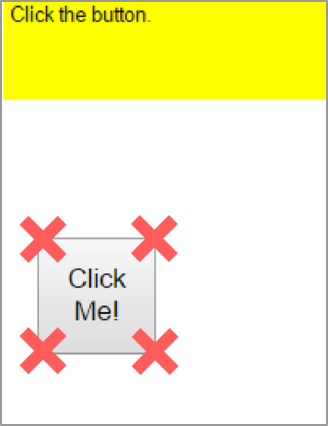
\includegraphics[width=0.9\columnwidth]{edge.png}
	\end{minipage}}
	\subfloat{%
	
\includegraphics[width=1.25in]{fov.png}}\quad
	\caption{Screen shots of different input processing techniques}
\end{figure}

Figure 2 presents three screenshots that showcases some of these experimented additions. The top left is a grayscaled and downsampled image to 84x84 pixels. Additionally, the key factor to this is that the last four frames before the current state are stacked into one image to provide directional information. The right image also uses a downsample view of the canvas. This method however makes use of an additional field-of-view, or a sort of \textit{"second eyesight"} that has a magnified view of the cursor up-close that also follows its movement. The bottom-right presents an illustration for an implementation of edge detection using the SciKit-Image library. This edge data is embedded within the pixel information in hopes to identify features (buttons, checkboxes, etc.) within the canvas more efficiently. All these processing techniques all have a general aim of providing an increased supervision to the agent in hopes of speeding up the training process.

\subsection{Implemented models}
One way to optimize the agents in this environment is to use on-policy and off-policy methods. On-policy methods create a policy to make decision that is being improved using the agent��s action value over time. Off-policy method is more complicated in which the agent (in the context of Q-Learning) is using a second greedy policy to determine the value of its actions, regardless of what the current policy recommends \cite{sutton1998reinforcement}. The chosen models for both methods are Policy Gradient and DDQN \& DDDQN for on-policy and off-policy respectively. 
\\\\
\underline{\bf On-policy methods}  
\\
Different action for each agent produces different rewards. One action may grant the agent positive reward if it'��s the correct move or negative reward if it'��s the incorrect move. In the on-policy method, we make sure the agent learns how to create a policy by choosing the optimal solution over time. There are multiple methods that implement an on-policy approach, however we are going to focus on one of the widely-used approaches, policy gradient.
\subsubsection{Policy Gradient}
Policy gradient is an on-policy method where the specified neural network is trained to create a policy by selecting optimal actions through gradient descent. Policy gradient implements a stochastic policy:
\[ \mu(a|s) \]
where:
\indent
\begin{itemize}
\item \({{a}}\) : action that the agent takes.
\item \({{s}}\) : state which the agent is experiencing.
\end{itemize}

This determines a probability distribution for the agent's actions throughout the training process. In the perfect world, the agent detects the wrong action with negative reward and detects the correct action with positive reward. Then after several trainings, the agent will be able to increase the chance of choosing the correct action. In the Mini World of Bits benchmark, the goal is to move the cursor to the specified target (button or text box) as close as possible and reward the agent if it manages to hit the button and learn from the chosen action'��s reward. 
\\In this research, the vanilla Policy Gradient was chosen as the main on-policy approach. To get a basic vanilla Policy Gradient to work, we had to do some visual manipulation to the state and use discrete action spaces with a Convolutional Neural Network (CNN) as the policy. At first, we tried to use a fully connected network as the policy, however the network has too many parameters and is more difficult to train whereas CNN considers neighbouring pixels to shrink down the calculation time and space.
\\\\
\underline{\bf Off-policy methods}  
\\
\subsubsection{Q Learning}
When we consider off-policy Temporal Difference (TD) control, a common method is through Q-Learning. Q Learning comprises of an action-value function that, when optimized, assists to find an optimal action-selection policy for a discrete MDP (this is where the compatibility for discrete action spaces come into play). This is through selection of actions with the highest Q value at a given state in time. In a formal sense, the Q function can be defined as :
\begin{align*}
Q\left( \mbox{S}_{t},\; A_{t} \right)\; &\leftarrow\;Q\left( \mbox{S}_{t},\; A_{t} \right)\;\\ 
&+\; \alpha_{t}\left[ R_{t+1}\; +\; \gamma \max _{a}Q\left( \mbox{S}_{t+1},\; A \right)\; -\; Q\left( \mbox{S}_{t},\; A_{t} \right) \right]
\end{align*}
We shall break down this equation as follows :
\indent
\begin{itemize}
\item \({{S}}_{{t}}\) : The state at a given time \textit{t}.
\item \({{A}}_{{t}}\) : The action performed on state S at time \textit{t}.
\item \({{\alpha}}_{{t}}\) : The learning rate (or step size). This is initially set to 1 and slowly converges to a value close to 0. This rate determines to what extent is the Q function still learning and changes to its policy. Once it converges to its designed minimum, the agent will not continue to learn.
\item \({{R}}_{{t+1}}\) : The Reward obtained from a given time \textit{t+1}
\item \({\gamma}\) : The discount factor. This is a set constant between the range of 0 to 1, and this determines to what extent future rewards are taken into consideration. For example, a \(\gamma\) of 0 means future rewards are neglected, whereas a \(\gamma\) of 1 means future rewards matter.
\item \(\max _{a}Q\left( \mbox{S}_{t+1},\; A \right)\) : This retrieves the Q-value of the action with the highest value within a set of actions \textit{A} for state \textit{S}
\end{itemize}

This Q-Learning function is iterated through every episode in the environment to eventually slowly converge to an optimal policy.

\subsubsection{Deep Q Learning}
The problem with such naive-iteration is that due to the dynamic nature of the environments, this can present a large scope of state-action pairs without any form of generalization, and the nature of iterating through each state-action pair for a given state is highly impractical. There is also the caveat where slight changes to the Q-values can result in significant changes to the policy that can diverge the optimization of the Q function. In such a case, we refer to a neural network as a function approximator with weights \(\theta\) to help stabilize estimations of the action-value function. This form of agent is referred to as a \textbf{Deep Q Network}\cite{deepqlearning}, serving as the primary architecture of our off-policy implementation. There are three main components to the Deep Q Network as follows:
\begin{itemize}
\item \textbf{Experience Replay} : Before the training process, an agent stores its experiences during each time step \textit{e(t)} in the form of a tuple represented as (\({{S}}_{{t}}\), \({{A}}_{{t}}\), \({{R}}_{{t+1}}\), \({{S}}_{{t+1}}\), \(d\)), with \(d\) a boolean variable signifying if the step completes the episode. These tuples are all stored in a replay memory \(D\) for a certain initial capacity. When the training process begins, the agent samples a batch of tuples from \(D\) that is fed onto a multi-layered neural network calculate predictions and update the Q-function for every \textit{e(t)}.\linebreak

\item \textbf{Convolutional Neural Network} : 
The main Q-network adapts the model of a Convolutional Neural Network (CNN). This performs feed-forward operations by reading through the pixel information stored within the tuples, performing calculations over a series of convolution layers with a final output of Q-values over a set of actions \(A\). It is using this CNN that interprets a generalization to the state-action pairs by updating through the weight parameters \(\theta\).\linebreak

\item \textbf{Target Network} :
We make use of a secondary neural network that is nothing more than a duplicate of the Q-Network mentioned above, but with its parameters \(\theta\) copied over a cycle of n number of steps. The Q-values produced from this network is used to assist with computation of the Loss function. For a target network with parameters \(\theta ^{-}\) and Q-network with parameters \(\theta\), the target value is defined as follows :
\begin{align*}
T_{DQN}\; = ( R\; +\; \lambda \max _{a}Q\left( \mbox{S}_{t+1},\; A_{t+1},\; \theta ^{-} \right)
\end{align*}

With the loss function defined as follows:
\begin{align*}
L\left( \theta  \right)\; =\; \mbox{E}_{\mbox{S},A,\mbox{S}_{t+1},R,D}\; \cdot \; \left[ \left(T_{DQN}\; -\; Q\left( \mbox{S},\; A,\; \theta  \right) \right)^{2}\right]
\end{align*}
This target network assists with stabilizing the convergence of the Q-values.
\end{itemize}

\subsubsection{Dueling Deep Q Learning}
The only difference to this architecture is that the single output layer from the CNN is explicitly split into two streams (state-value and advantage), which is then re-combined using an equation to produce the final prediction for a set of actions \(A\). The rest of the Reinforcement Learning architecture remains intact.

\begin{figure}[h!]
\centering
	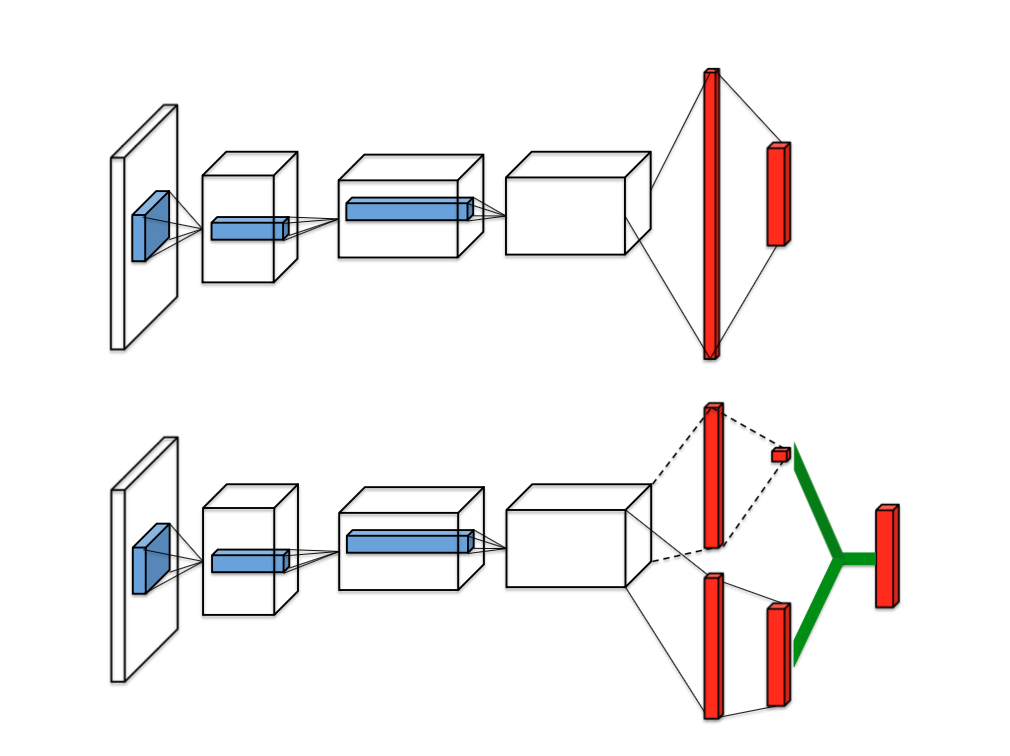
\includegraphics[width=0.7\columnwidth, keepaspectratio]{dueling.png}
	\caption{A visual illustration comparing the regular DQN (top) and Dueling DQN \cite{dueling} (bottom)}
	\label{fig:dueling}
\end{figure}

\subsubsection{Double Deep Q Learning}
One feature of the DQN uses a max operator to select and evaluate actions upon a given state with the target network. The problem with this approach is that this can lead to selection of overestimated values, which can delay the time in learning the optimal policy. A simple fix to this, referred to as the Double Deep Q-Network \cite{doubledeepqlearning}, uses a different equation to update the target value :
\begin{align*}
T_{DDQN}\; =\; R\; +\; \lambda Q\left( \mbox{S}_{t+1},\; \mbox{argmax}Q\left( \mbox{S}_{t+1},\; a,\; \theta ^{-} \right),\; \theta ^{-} \right)
\end{align*}

\subsection{Reward manipulation}
The current reward system for any given environment follows the agenda that if the agent completes the designated task within a certain time limit, it receives a positive reward signal between 0 to 1 (depending on how much time was remaining). Otherwise, it would receive a negative reward signal of -1 if the agent fails to complete the task on time. \linebreak

One approach we looked into are additional reward manipulation techniques added to the above reward signals in hopes to improve the efficiency of the training process. One caveat to be aware of in regards to these environments is that during the learning process, there is the possibility for a sequence of actions that can result in the cursor moving outside the canvas area onto an irrelevant space. While we can simply add logical expression to not take any action if the cursor were to reach the edge of the canvas, it may not directly learn from this caveat due to a lack of error signal of any sort. As a result, if the cursor is located at an edge and performs an action that would result in the cursor moving outside the canvas, it would receive a negative reward signal of -0.1 deducted from the cumulative reward. \linebreak

Inversely, we also try to provide positive reward signals if the cursor performed progressive steps towards completion of the task. For example, one of the environments involved clicking a randomly generated button within the canvas. One of the algorithms keep record of the current position of the generated button, and sets up a proximity area around the button, for if the button were to perform an action that would result in the position of the cursor to move closer towards the button, would in turn receive a positive reward signal of +0.1 added to the final cumulative reward. \linebreak

\subsection{Supervised methods}

\subsection{Metrics}

\subsection{Training Setup}
The training procedure for these agents were primarily run over a server that comprised of an Nvidia TITAN X GPU. We compiled and installed the TensorFlow library to take advantage of additional CPU instructions (SSE4.2,AVX2 and FMA), as well as additional GPU capabilities, such as the Nvidia CUDA platform. These optimizations were to ensure we were reaching as much benefit of performance enhancements as possible for added efficiency to training. The results of all our agents were logged and visualized using the in-built TensorBoard to analyze performance of the agents

\subsection{Benchmarks}

\section{Results}

\section{Analysis}

\subsection{Limitations}

\section{Conclusion and future work}
\subsection{Conclusion}
Following from the analysis of our results, we can conclude that...
\subsection{Future work}
The novelty of the benchmark indicates still a wide area of progress that can be made, as such there are many future possibilities to expand upon the current state of our project:
\subsubsection{Continuous action spaces}
As we have only discussed discrete action spaces, we would invest more research into implementing continuous action spaces. We are still currently looking into the full implementation and training of an agent via a \textbf{Deep Deterministic Policy Gradient} algorithm \cite{lillicrap2015continuous}, which is specifically designed for continuous action spaces and has shown to be very effective in other non-MWoB environments that use continuous actions, such as the inverted pendulum experiment \cite{pendulum} where the objective is to provide a magnitude to balance the pendulum. The algorithm focuses on an actor-critic method, where the policy function structure is known as the actor, and the value function structure is known as the critic. The actor produces an action given the current state of the environment, and the critic produces a Temporal-Difference error signal given the state and resultant reward. Both the actor and critic learn from the critic's output. In this scenario, neural networks can be used to represent the actor and critic structures, more specifically convolutional neural networks.

We have looked at modelling a magnitude of an action space ranging from -1 to 1 for both angle and distance, where the magnitude is then scaled into a discretised action. This differs to existing solutions which only produce one magnitude for an action. The simple equation below shows how the angle in radians, \( \theta \), is calculated via magnitude \textit{m}:
\[ \theta=m\pi \]
For example, if magnitude was -0.5, the angle to move would be -\( 0.5\pi \). A similar equation would be used to scale the distance \textit{d} by a set fixed distance \textit{D}:
\[ d=mD \]
 Following this, the \textit{x} and \textit{y} distances to move can be calculated accordingly:
 \[ xdist=dsin\theta \]
 \[ ydist=dcos\theta \]
 
This method could prove to be more effective than existing methods that we have implemented due to the fact that hypothetically it would learn quicker; the mouse can navigate to anywhere within the canvas in one step instead of a discretised action space where it would have to slowly navigate to a designated area via several steps.

\subsubsection{Natural language processing}
Another development would be performing natural language processing on the webpage. To elaborate on this with an example, if the question told us to enter a certain word into a text box, we would need NLP to identify this in the prompt in accordance with the agent to correspond with the features identified in the canvas. This can further be extended by analysing the vision to find relevant text via two possible methods:
\indent
\begin{itemize}
\item Optical Character Recognition (OCR) - identify and convert webpage text into machine-encoded text. This is eased by the fact that we are already performing input processing on the image fed to the agent, such that pre-processes in OCR such as binarisation are not needed. 
\item Analysing Document Object Models (DOM) - identify key elements in the webpage where text is concerned. This would further be able to split up certain elements and attempt to classify them for the agent, such as identifying date inputs.
\end{itemize}

\subsubsection{Categorical tasks}
As we have only experimented on environments where clicking an object is the goal of the task, it would be ideal to expand further to other categories of environments, such as dragging and dropping tasks or text-input tasks. Some more complex tasks within the benchmark involve using a combination of these categories e.g drag and drop an object into an area and click submit. It is highly possible that once most, if not all, of the task categories are fulfilled/trained, the agent would be able to train successfully on real-world websites that involve these respective tasks.


% use section* for acknowledgment
%\section*{Acknowledgment}


%The authors would like to thank...

% to add a reference, go to the article page and find the option to 'cite' via BibTex. Copy and paste this into the .bib file and make note of the citation key (change the citation key to something easier to remember for yourself if you want), and then use \cite{citationkey} where you want to reference. You need to compile the bibliography before it will show (Command+shift+B on mac), then compile normally and your reference should show correctly. 

\bibliography{references}
\bibliographystyle{IEEEtran}



% that's all folks
\end{document}


